\section{Complete Upgrade Effects and Their Interpretation}
\label{app:tables}

This appendix supports \S\ref{sec:value}: replacing a W4 agent's action produces both rescues and damages, and a gain measured for one upgrade mode cannot be reused as the gain of another.

Table~\ref{tab:r1} expands Figure~\ref{fig:rd}a and adds the stress configurations, with both interval types. Table~\ref{tab:ghf} reports $G$, $H$, $F$ and $G-H$; Table~\ref{tab:ghf-patterns} adds $F-G$, $F-H$ and the outcome-pattern summaries. % nocheck: cross-reference sentence

\begin{figure*}[t]
\centering
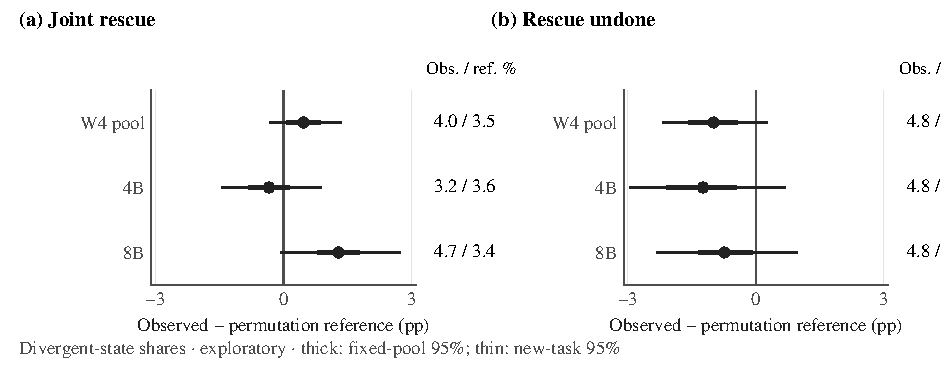
\includegraphics[width=\textwidth]{figures/f14_pattern_reference.pdf}
\caption{Joint rescue and rescue undone relative to label permutation on W4 divergent states. Thick lines show fixed-pool 95\% intervals; thin lines show new-task 95\% intervals. The right columns give observed and reference shares. These exploratory comparisons test enrichment, separately from the observed pattern counts in the main text. Values: Table~\ref{tab:patternref}.} % nocheck: interval conventions copied from the original caption; no outcome estimates here
\label{fig:modesfull}
\label{fig:modes}
\end{figure*}

\begin{table*}[t]
\centering% visual-layout-v1
\renewcommand{\arraystretch}{1.12}\fontsize{8.5}{10}\selectfont\setlength{\tabcolsep}{4pt}
% src: analysis/fork/out/dev_all_20261001T070326Z.md (two-sided table; W4:all pooled row); analysis/fork/out/dev_all_20261001T070326Z.json (pooled.W4:all:pooled_equal_weight.G.crossed_ci95)
\begin{tabular}{@{}lrrrrrll@{}}
\toprule
Cell & units & div. & $r$ & $d$ & $M$ & $\Gall$ [fixed pool] & [new tasks] \\
\midrule
q4 GPTQ-W4 & 85$\times$20 & 1102 & 6.8 & 8.7 & 15.5 & $-1.9$ [$-3.7$, $-0.1$] & [$-6.8$, $+2.7$] \\
q4 AWQ-style W4  & 85$\times$20 & 1439 & 9.8 & 10.1 & 19.9 & $-0.3$ [$-2.2$, $+1.6$] & [$-5.4$, $+5.2$] \\
q8 GPTQ-W4 & 85$\times$20 & 1473 & 10.4 & 7.5 & 17.9 & $+2.9$ [$+1.4$, $+4.4$] & [$-2.9$, $+9.2$] \\
q8 AWQ-style W4  & 85$\times$20 & 1562 & 11.4 & 9.5 & 20.9 & $+1.9$ [$-0.6$, $+4.3$] & [$-3.9$, $+8.1$] \\
W4 pool    & 85$\times$20 & & 9.6 & 9.0 & 18.6 & $+0.7$ [$-0.3$, $+1.6$] & [$-2.1$, $+3.4$] \\
\midrule
q4 KV8 & 85$\times$22 & 593 & 3.1 & 3.4 & 6.5 & $-0.3$ [$-1.7$, $+1.0$] & [$-3.0$, $+2.3$] \\
q8 KV8 & 85$\times$22 & 855 & 4.3 & 3.7 & 8.1 & $+0.6$ [$-0.4$, $+1.6$] & [$-1.9$, $+3.0$] \\
\midrule
q4 GPTQ-W3$^s$ & 85$\times$3 & 232 & 9.0 & 10.2 & 19.2 & $-1.2$ [$-7.0$, $+4.7$] & [$-8.6$, $+5.9$] \\
q4 KV4-rot$^s$ & 85$\times$3 & 233 & 11.8 & 7.1 & 18.8 & $+4.7$ [$-4.1$, $+13.5$] & [$-3.1$, $+12.9$] \\
q8 GPTQ-W3$^s$ & 85$\times$3 & 242 & 10.2 & 8.2 & 18.4 & $+2.0$ [$-12.5$, $+16.4$] & [$-6.3$, $+11.8$] \\
q8 KV4-rot$^s$ & 85$\times$3 & 239 & 11.8 & 8.6 & 20.4 & $+3.1$ [$-14.5$, $+20.8$] & [$-5.9$, $+12.9$] \\
q8 RTN-W3$^s$ & 85$\times$3 & 255 & 3.1 & 3.5 & 6.7 & $-0.4$ [$-3.8$, $+3.0$] & [$-4.7$, $+3.9$] \\
\bottomrule
\end{tabular}
\caption{Replacing Q's first tool-structure-divergent action while Q continues, \tautwo{} retail/airline panel (pp). Denominator: the full pool of tasks $\times$ complete blocks; units without a Bank P state count as zero. div.\ = Bank P states. $\Gall=r-d$ is a local replacement effect, \emph{not} the end-to-end success difference (Appendix~\ref{app:e2e}). Fixed pool: block bootstrap ($\ge$10 blocks) or $t$ over block means; new tasks: crossed task$\times$block bootstrap. $^s$stress cell, 3 blocks.}
\label{tab:r1}
\end{table*}

% GENERATED by tools/gen_ghf_combined.py; display only, no analysis changes.
% src: analysis/fork/out/ghf_20261001T211519Z.json; analysis/fork/out/ghf_20261001T211519Z.md; analysis/fork/out/ghf_multiplicity_20261001T225727Z.md
\begin{table*}[t]
\centering\fontsize{9}{11}\selectfont
\renewcommand{\arraystretch}{1.15}\setlength{\tabcolsep}{4pt} % nocheck: layout
\begin{tabular*}{\textwidth}{@{\extracolsep{\fill}}llllll@{}}
\toprule
Cell & states & $G$ (action) & $H$ (continuation) & $F$ (joint) & $G-H$ \\
\midrule
q4 GPTQ-W4 & 1102 & \shortstack[l]{$-2.9$ [$-5.7$, $-0.2$]\\{}[$-10.3$, $+4.2$]} & \shortstack[l]{$+0.7$ [$-1.6$, $+3.0$]\\{}[$-4.0$, $+6.0$]} & \shortstack[l]{$-2.5$ [$-5.3$, $+0.2$]\\{}[$-9.9$, $+4.7$]} & \shortstack[l]{$-3.6$ [$-6.6$, $-0.6$]\\{}[$-11.2$, $+3.6$]} \\
\addlinespace[1pt] % nocheck: layout
q4 AWQ-style W4 & 1439 & \shortstack[l]{$-0.3$ [$-2.6$, $+1.9$]\\{}[$-6.5$, $+6.1$]} & \shortstack[l]{$+0.9$ [$-1.1$, $+2.9$]\\{}[$-3.7$, $+5.5$]} & \shortstack[l]{$-0.8$ [$-3.3$, $+1.6$]\\{}[$-7.4$, $+5.8$]} & \shortstack[l]{$-1.3$ [$-3.0$, $+0.6$]\\{}[$-7.7$, $+5.1$]} \\
\addlinespace[1pt] % nocheck: layout
q8 GPTQ-W4 & 1473 & \shortstack[l]{$+3.3$ [$+1.6$, $+5.0$]\\{}[$-3.3$, $+10.5$]} & \shortstack[l]{$+0.4$ [$-1.2$, $+1.9$]\\{}[$-3.8$, $+4.9$]} & \shortstack[l]{$+5.4$ [$+3.5$, $+7.2$]\\{}[$-2.0$, $+13.0$]} & \shortstack[l]{$+2.9$ [$+1.3$, $+4.7$]\\{}[$-3.2$, $+9.3$]} \\
\addlinespace[1pt] % nocheck: layout
q8 AWQ-style W4 & 1562 & \shortstack[l]{$+2.1$ [$-0.6$, $+4.7$]\\{}[$-4.1$, $+8.7$]} & \shortstack[l]{$-1.3$ [$-3.5$, $+0.9$]\\{}[$-7.1$, $+4.6$]} & \shortstack[l]{$+0.6$ [$-1.5$, $+2.7$]\\{}[$-6.2$, $+7.3$]} & \shortstack[l]{$+3.4$ [$+1.5$, $+5.2$]\\{}[$-1.6$, $+8.6$]} \\
\addlinespace[1pt] % nocheck: layout
W4 pool & 5576 & \shortstack[l]{$+0.5$ [$-0.7$, $+1.7$]\\{}[$-2.9$, $+3.8$]} & \shortstack[l]{$+0.2$ [$-1.3$, $+1.6$]\\{}[$-2.7$, $+2.8$]} & \shortstack[l]{$+0.7$ [$-0.6$, $+2.1$]\\{}[$-3.1$, $+4.4$]} & \shortstack[l]{$+0.4$ [$-0.8$, $+1.7$]\\{}[$-3.1$, $+3.7$]} \\
\addlinespace[1pt] % nocheck: layout
\midrule
q4 KV8 & 593 & \shortstack[l]{$-1.0$ [$-5.3$, $+3.2$]\\{}[$-9.4$, $+7.3$]} & \shortstack[l]{$-2.5$ [$-4.5$, $-0.5$]\\{}[$-6.4$, $+1.1$]} & \shortstack[l]{$-1.2$ [$-4.7$, $+2.3$]\\{}[$-9.3$, $+7.7$]} & \shortstack[l]{$+1.5$ [$-3.1$, $+6.0$]\\{}[$-7.1$, $+9.7$]} \\
\addlinespace[1pt] % nocheck: layout
q8 KV8 & 855 & \shortstack[l]{$+1.3$ [$-0.9$, $+3.4$]\\{}[$-4.0$, $+6.9$]} & \shortstack[l]{$-0.4$ [$-2.1$, $+1.5$]\\{}[$-3.5$, $+2.9$]} & \shortstack[l]{$+2.5$ [$+0.0$, $+5.1$]\\{}[$-3.5$, $+8.1$]} & \shortstack[l]{$+1.6$ [$-0.6$, $+3.9$]\\{}[$-3.8$, $+7.2$]} \\
\addlinespace[1pt] % nocheck: layout
KV8 pool & 1448 & \shortstack[l]{$+0.1$ [$-2.8$, $+3.0$]\\{}[$-5.3$, $+5.6$]} & \shortstack[l]{$-1.4$ [$-2.7$, $-0.1$]\\{}[$-3.7$, $+0.9$]} & \shortstack[l]{$+0.6$ [$-1.8$, $+3.1$]\\{}[$-4.5$, $+5.8$]} & \shortstack[l]{$+1.6$ [$-1.2$, $+4.1$]\\{}[$-3.8$, $+6.6$]} \\
\addlinespace[1pt] % nocheck: layout
\midrule
q4 GPTQ-W3$^s$ & 232 & \shortstack[l]{$-1.3$ [$-7.7$, $+5.0$]\\{}[$-9.7$, $+6.6$]} & \shortstack[l]{$+4.3$ [$-10.7$, $+19.4$]\\{}[$-6.6$, $+14.5$]} & \shortstack[l]{$+1.3$ [$-1.9$, $+4.4$]\\{}[$-6.8$, $+9.4$]} & \shortstack[l]{$-5.6$ [$-15.0$, $+3.7$]\\{}[$-15.0$, $+4.0$]} \\
\addlinespace[1pt] % nocheck: layout
q4 KV4-rot$^s$ & 233 & \shortstack[l]{$+5.2$ [$-4.5$, $+14.9$]\\{}[$-3.4$, $+14.2$]} & \shortstack[l]{$+9.4$ [$+5.1$, $+13.7$]\\{}[$+2.1$, $+17.0$]} & \shortstack[l]{$+12.4$ [$+11.0$, $+13.9$]\\{}[$+3.0$, $+21.6$]} & \shortstack[l]{$-4.3$ [$-18.3$, $+9.8$]\\{}[$-13.5$, $+7.0$]} \\
\addlinespace[1pt] % nocheck: layout
q8 GPTQ-W3$^s$ & 242 & \shortstack[l]{$+2.1$ [$-13.3$, $+17.2$]\\{}[$-6.7$, $+12.1$]} & \shortstack[l]{$+0.4$ [$-7.4$, $+8.2$]\\{}[$-7.2$, $+8.1$]} & \shortstack[l]{$+2.1$ [$-7.4$, $+11.4$]\\{}[$-6.6$, $+11.8$]} & \shortstack[l]{$+1.7$ [$-9.1$, $+12.3$]\\{}[$-7.7$, $+11.2$]} \\
\addlinespace[1pt] % nocheck: layout
q8 KV4-rot$^s$ & 239 & \shortstack[l]{$+3.3$ [$-15.4$, $+21.9$]\\{}[$-6.6$, $+13.8$]} & \shortstack[l]{$-0.8$ [$-18.2$, $+16.3$]\\{}[$-11.2$, $+8.5$]} & \shortstack[l]{$+4.6$ [$-16.0$, $+25.0$]\\{}[$-6.6$, $+15.9$]} & \shortstack[l]{$+4.2$ [$+2.5$, $+5.8$]\\{}[$-3.3$, $+12.2$]} \\
\addlinespace[1pt] % nocheck: layout
q8 RTN-W3$^s$ & 255 & \shortstack[l]{$-0.4$ [$-3.8$, $+3.0$]\\{}[$-4.7$, $+3.9$]} & \shortstack[l]{$+15.3$ [$+0.7$, $+29.9$]\\{}[$+5.9$, $+25.9$]} & \shortstack[l]{$+18.4$ [$+16.7$, $+20.1$]\\{}[$+9.4$, $+28.2$]} & \shortstack[l]{$-15.7$ [$-27.5$, $-3.9$]\\{}[$-24.7$, $-7.1$]} \\
\addlinespace[1pt] % nocheck: layout
\bottomrule
\end{tabular*}
\caption{Upgrade gains on divergent states (pp). In each two-line cell, the first line gives the estimate and fixed-pool 95\% interval; the second gives the new-task crossed 95\% interval. $G$, $H$ and $F$ compare action-only, continuation-only and joint replacement with QQ. Fixed-pool intervals use a block bootstrap over 20--22 blocks, or a $t$ interval over three blocks for $^s$stress configurations. Pools average within-configuration estimates equally; stress configurations are separate.}
\label{tab:ghf}
\label{tab:ghf-crossed}
\end{table*}

% GENERATED by tools/gen_ghf_combined.py; display only, no analysis changes.
% src: analysis/fork/out/ghf_20261001T211519Z.json; analysis/fork/out/ghf_20261001T211519Z.md; analysis/fork/out/ghf_multiplicity_20261001T225727Z.md
\begin{table*}[t]
\centering\fontsize{9}{11}\selectfont
\renewcommand{\arraystretch}{1.15}\setlength{\tabcolsep}{4pt} % nocheck: layout
\begin{tabular*}{\textwidth}{@{\extracolsep{\fill}}llllll@{}}
\toprule
Cell & $F-G$ & $F-H$ & off-diag.\ \% & rev.\ \% & mean $I$ \\
\midrule
q4 GPTQ-W4 & \shortstack[l]{$+0.5$ [$-1.2$, $+2.2$]\\{}[$-4.7$, $+6.1$]} & \shortstack[l]{$-3.2$ [$-6.4$, $+0.2$]\\{}[$-11.1$, $+4.4$]} & 25.0 & 2.6 & $+0.3$ \\
\addlinespace[1pt] % nocheck: layout
q4 AWQ-style W4 & \shortstack[l]{$-0.4$ [$-2.4$, $+1.5$]\\{}[$-6.2$, $+5.4$]} & \shortstack[l]{$-1.7$ [$-3.6$, $+0.4$]\\{}[$-8.7$, $+4.7$]} & 29.3 & 3.1 & $+1.3$ \\
\addlinespace[1pt] % nocheck: layout
q8 GPTQ-W4 & \shortstack[l]{$+2.1$ [$+0.2$, $+4.0$]\\{}[$-3.0$, $+7.1$]} & \shortstack[l]{$+5.0$ [$+3.2$, $+6.8$]\\{}[$-2.0$, $+12.5$]} & 22.9 & 2.7 & $-1.7$ \\
\addlinespace[1pt] % nocheck: layout
q8 AWQ-style W4 & \shortstack[l]{$-1.5$ [$-4.2$, $+0.8$]\\{}[$-7.6$, $+4.2$]} & \shortstack[l]{$+1.9$ [$-0.1$, $+3.8$]\\{}[$-3.8$, $+7.5$]} & 30.5 & 4.2 & $+0.3$ \\
\addlinespace[1pt] % nocheck: layout
W4 pool & \shortstack[l]{$+0.2$ [$-1.0$, $+1.2$]\\{}[$-2.8$, $+3.1$]} & \shortstack[l]{$+0.5$ [$-1.0$, $+2.1$]\\{}[$-3.5$, $+4.5$]} & 26.9 & 3.2 & $+0.0$ \\
\addlinespace[1pt] % nocheck: layout
\midrule
q4 KV8 & \shortstack[l]{$-0.2$ [$-3.5$, $+3.7$]\\{}[$-5.7$, $+5.3$]} & \shortstack[l]{$+1.3$ [$-2.5$, $+4.9$]\\{}[$-6.7$, $+9.5$]} & 15.7 & 1.2 & $-2.4$ \\
\addlinespace[1pt] % nocheck: layout
q8 KV8 & \shortstack[l]{$+1.2$ [$-0.5$, $+3.2$]\\{}[$-2.5$, $+5.0$]} & \shortstack[l]{$+2.8$ [$+0.3$, $+5.5$]\\{}[$-3.1$, $+8.7$]} & 14.9 & 1.2 & $-1.5$ \\
\addlinespace[1pt] % nocheck: layout
KV8 pool & \shortstack[l]{$+0.5$ [$-1.6$, $+2.8$]\\{}[$-2.8$, $+3.9$]} & \shortstack[l]{$+2.1$ [$-0.2$, $+4.2$]\\{}[$-3.0$, $+7.3$]} & 15.3 & 1.2 & $-1.9$ \\
\addlinespace[1pt] % nocheck: layout
\midrule
q4 GPTQ-W3$^s$ & \shortstack[l]{$+2.6$ [$-0.6$, $+5.8$]\\{}[$-5.2$, $+10.5$]} & \shortstack[l]{$-3.0$ [$-15.1$, $+9.1$]\\{}[$-12.2$, $+6.6$]} & 31.5 & 3.9 & $+1.7$ \\
\addlinespace[1pt] % nocheck: layout
q4 KV4-rot$^s$ & \shortstack[l]{$+7.3$ [$-2.0$, $+16.5$]\\{}[$-1.3$, $+17.1$]} & \shortstack[l]{$+3.0$ [$-1.9$, $+8.0$]\\{}[$-6.2$, $+12.2$]} & 33.0 & 1.7 & $+2.1$ \\
\addlinespace[1pt] % nocheck: layout
q8 GPTQ-W3$^s$ & \shortstack[l]{$+0.0$ [$-11.0$, $+11.1$]\\{}[$-9.1$, $+9.1$]} & \shortstack[l]{$+1.7$ [$-0.1$, $+3.4$]\\{}[$-6.8$, $+11.0$]} & 23.1 & 4.5 & $+0.4$ \\
\addlinespace[1pt] % nocheck: layout
q8 KV4-rot$^s$ & \shortstack[l]{$+1.3$ [$-1.8$, $+4.3$]\\{}[$-7.2$, $+9.9$]} & \shortstack[l]{$+5.4$ [$+0.8$, $+10.0$]\\{}[$-2.5$, $+14.6$]} & 31.0 & 4.6 & $-2.1$ \\
\addlinespace[1pt] % nocheck: layout
q8 RTN-W3$^s$ & \shortstack[l]{$+18.8$ [$+13.8$, $+23.9$]\\{}[$+10.2$, $+27.8$]} & \shortstack[l]{$+3.1$ [$-13.0$, $+19.2$]\\{}[$-7.1$, $+13.3$]} & 29.0 & 0.4 & $-3.5$ \\
\addlinespace[1pt] % nocheck: layout
\bottomrule
\end{tabular*}
\caption{Paired mode contrasts and outcome patterns on the states of Table~\ref{tab:ghf}. Two-line cells give fixed-pool and new-task 95\% intervals in that order. Off-diag.: $\DQ\ne\DB$; rev.: $\DQ=-\DB\ne0$; interaction $I=\DQ-\DB$. Intervals are unadjusted. The four core W4 $G-H$ tests form a Holm family: q4 GPTQ-W4 has adjusted $p=.069$; all four new-task intervals cover zero. A positive $G-H$ compares two upgrades, not either upgrade against QQ.}
\label{tab:ghf-patterns}
\end{table*}



\label{app:r2main}

\subsection{The Two Illustrative Rescue Patterns} % nocheck: heading
\label{app:offdiag}

Everything in this section is exploratory and post hoc. It uses the four outcomes of each divergent state in the order BB, BQ, QB, QQ; $k$ is the number of successful arms.

\paragraph{Joint rescue and rescue undone against the reference.} A label-permutation reference for the two named patterns keeps $k$ for every state and permutes the four outcome labels uniformly: \texttt{1000} then has probability $1/4$ at $k=1$, and rescue undone (\texttt{0100} or \texttt{0110}) has $1/4$ at $k=1$ plus $1/6$ at $k=2$, so the reference shares are $P(k{=}1)/4$ and $P(k{=}1)/4+P(k{=}2)/6$, computed on the same states and bootstrap draws as the observed shares (Table~\ref{tab:patternref}). In the \tautwo{} W4 pool, joint rescue exceeds the reference by $+0.47$\pp{} on the fixed task pool ([$+0.06$, $+0.87$]), but the new-task interval spans zero ([$-0.33$, $+1.37$]); rescue undone is less frequent than the reference ($-0.99$ [$-1.58$, $-0.42]$; new tasks [$-2.19$, $+0.27$]). The excess of joint rescue is concentrated in the q8 cells, and no group shows a new-task excess of rescue undone. Because the reference keeps $k$ and does not model execution, a share near it says that the arrangement is about as common as a random arrangement of the same number of successes, not that the outcomes are noise or that the continuation is irrelevant. % src: analysis/fork/out/pattern_ref_20261005T134721Z.md (TL;DR; §1; §2; Method)
The observed shares in the W4 pool, with both intervals, are 4.0\% for joint rescue (fixed pool [3.5, 4.5]; new tasks [2.7, 5.3]) and 4.8\% for rescue undone ([4.1, 5.4]; [3.2, 6.5]). % src: analysis/fork/out/outcome_classes_20261004T143614Z.md (TL;DR; pool W4:all rows)

\begin{table*}[t]
\centering% visual-layout-v1
\renewcommand{\arraystretch}{1.12}\fontsize{8.5}{10}\selectfont\setlength{\tabcolsep}{4pt}
% src: analysis/fork/out/pattern_ref_20261005T134721Z.md (§1 fixed pool; §2 new tasks); analysis/fork/out/mistral_patterns_20261005T135040Z.md (§4, §5: A6:nonexact:pool)
\begin{tabular*}{\textwidth}{@{\extracolsep{\fill}}llllll@{}}
\toprule
\multicolumn{6}{@{}l}{\textbf{A. Joint rescue}} \\
\addlinespace[2pt]
Group & states & obs. & ref. & obs.$-$ref.\ [fixed pool] & [new tasks] \\
\midrule
\tautwo{} W4 pool & 5576 & 3.96 & 3.48 & $+0.47$ [$+0.06$, $+0.87$] & [$-0.33$, $+1.37$] \\
\quad q4 W4 cells & 2541 & 3.22 & 3.56 & $-0.34$ [$-0.83$, $+0.13$] & [$-1.46$, $+0.88$] \\
\quad q8 W4 cells & 3035 & 4.69 & 3.40 & $+1.29$ [$+0.79$, $+1.78$] & [$-0.07$, $+2.74$] \\
\tautwo{} KV8 pool & 1448 & 2.99 & 2.17 & $+0.81$ [$+0.10$, $+1.52$] & [$-0.51$, $+2.19$] \\
Telecom q8 W4 pool & 957 & 3.24 & 3.94 & $-0.70$ [$-1.46$, $+0.05$] & [$-2.47$, $+1.15$] \\
Same-precision W4 (Q$'$ as B) & 784 & 2.27 & 3.50 & $-1.23$ [$-2.47$, $-0.04$] & [$-2.88$, $+0.51$] \\
BF16, same blocks & 784 & 4.96 & 3.53 & $+1.43$ [$-0.40$, $+3.42$] & [$-0.90$, $+4.26$] \\
Mistral, own BF16 states$^m$ & 464 & 3.4 & 2.9 & $+0.5$ [$-2.4$, $+3.5$] & [$-2.0$, $+3.6$] \\
\bottomrule
\end{tabular*}
\par\vspace{6pt}
\begin{tabular*}{\textwidth}{@{\extracolsep{\fill}}llllll@{}}
\toprule
\multicolumn{6}{@{}l}{\textbf{B. Rescue undone}} \\
\addlinespace[2pt]
Group & states & obs. & ref. & obs.$-$ref.\ [fixed pool] & [new tasks] \\
\midrule
\tautwo{} W4 pool & 5576 & 4.80 & 5.78 & $-0.99$ [$-1.58$, $-0.42$] & [$-2.19$, $+0.27$] \\
\quad q4 W4 cells & 2541 & 4.77 & 6.01 & $-1.24$ [$-2.09$, $-0.45$] & [$-2.97$, $+0.69$] \\
\quad q8 W4 cells & 3035 & 4.82 & 5.56 & $-0.74$ [$-1.35$, $-0.07$] & [$-2.34$, $+0.98$] \\
\tautwo{} KV8 pool & 1448 & 2.31 & 4.58 & $-2.28$ [$-2.98$, $-1.58$] & [$-3.62$, $-0.98$] \\
Telecom q8 W4 pool & 957 & 4.18 & 5.13 & $-0.95$ [$-1.70$, $-0.20$] & [$-2.63$, $+0.61$] \\
Same-precision W4 (Q$'$ as B) & 784 & 5.77 & 5.75 & $+0.02$ [$-2.33$, $+2.25$] & [$-2.66$, $+2.92$] \\
BF16, same blocks & 784 & 3.82 & 6.14 & $-2.32$ [$-4.46$, $-0.19$] & [$-4.68$, $+0.17$] \\
Mistral, own BF16 states$^m$ & 464 & 4.0 & 4.7 & $-0.7$ [$-2.0$, $+0.7$] & [$-3.0$, $+1.9$] \\
\bottomrule
\end{tabular*}
\par\vspace{6pt}
\caption{Joint rescue and rescue undone against the conditional label-permutation reference (keeps the number $k$ of successful branches per state), \% of divergent states; exploratory, post hoc. 95\% intervals: fixed pool (block bootstrap for the 20- and 22-block \tautwo{} pools, $t$ over per-block ratios for fewer than 10 blocks: 6, or 5 for Mistral), new tasks (crossed task$\times$block). Same-precision rows each fork at their own first divergence. $^m$States whose actions differ, on BF16 trajectories (BB is the BF16 original), five blocks; not comparable with Bank P rows.}
\label{tab:patternref}
\end{table*}

\subsection{Task fragility}
\label{app:concentration}

All analyses in this subsection are exploratory and post hoc.

\paragraph{The consequences recur on the same tasks.} We split the 20 nonce blocks into two halves by an outcome-independent hash of the block name, ranked tasks by turnover on one half and measured the other half (Appendix Table~\ref{tab:fragility}). The 17 most fragile tasks (top 20\%) carry 41.0\% (crossed [26.6, 55.9]) and 42.3\% ([27.0, 57.5]) of the held-out turnover in the two directions, against 20\% if fragility did not persist. Their turnover is 38.7\%, while the other 68 tasks still turn over 13.7\%. Both groups have rescues and damages; neither group's net gain is resolved under the crossed interval. This replicates fragility on other nonces of the same tasks; it does not predict which new tasks are fragile. % src: analysis/fork/out/task_fragility_20261005T134836Z.md (Split-half fragility, both directions); analysis/fork/out/task_fragility_split_20261005T134815Z.json; derived: 68=85-17

\begin{table*}[t]
\centering% visual-layout-v1
\renewcommand{\arraystretch}{1.12}\fontsize{8.5}{10}\selectfont\setlength{\tabcolsep}{4pt}
% src: analysis/fork/out/task_fragility_20261005T134836Z.md (Split-half fragility: define A -> estimate B)
\begin{tabular}{@{}llllll@{}}
\toprule
Tasks & & $r$ & $d$ & $M$ & $\Gall$ \\
\midrule
fragile & est. & 21.1 & 17.6 & 38.7 & $+3.4$ \\
(top 20\%) & $t$ & [18.6, 23.5] & [14.3, 21.0] & [34.9, 42.6] & [$-1.0$, $+7.9$] \\
 & crossed & [14.8, 28.1] & [12.4, 23.3] & [32.3, 45.7] & [$-7.1$, $+13.7$] \\
\midrule
rest & est. & 6.5 & 7.2 & 13.7 & $-0.7$ \\
 & $t$ & [5.2, 7.8] & [6.2, 8.3] & [12.5, 14.9] & [$-2.7$, $+1.2$] \\
 & crossed & [4.4, 9.0] & [4.8, 9.9] & [10.2, 17.5] & [$-4.1$, $+2.4$] \\
\bottomrule
\end{tabular}
\caption{Repeatable task fragility (exploratory, post hoc; four \tautwo{} W4 cells, equal weight). Tasks are ranked by turnover on one hash-defined half of the 20 nonce blocks and measured on the other half (pp of units; 95\% intervals, $t$ over held-out blocks and crossed task$\times$block; direction A to B shown). A replication on other nonces of the same tasks, not a prediction for new tasks. Reverse direction: text.}
\label{tab:fragility}
\end{table*}

\paragraph{Split-half fragility (Table~\ref{tab:fragility}).} The halves are assigned by an outcome-independent hash of the block name (sha256 of a fixed prefix and the block name, mod 2), written to a file before this post hoc analysis loaded outcomes; fragility is a task's mean turnover over the four W4 cells and the defining half's blocks, and ties at the top-20\% threshold are broken by a hash. In the reverse direction (rank on the second half, estimate on the first), the 17 fragile tasks turn over 39.0\% ($t$ [34.2, 43.9]) and carry 42.3\% of the held-out turnover, the other tasks 13.3\%; the fragile tasks' net gain is $+3.7$\pp{} ($t$ [$+0.6$, $+6.9$]; crossed [$-5.0$, $+12.4$]) and the rest's $+0.5$. Ranking tasks by BF16 success instead (tertiles on one half) also separates turnover: the hardest tertile turns over 6.7--10.0\% and the others 25.4--27.3\%, with no net gain resolved under the crossed interval. % src: analysis/fork/out/task_fragility_20261005T134836Z.md (Split-half B -> A; BF16 difficulty tertiles; Method); analysis/fork/out/task_fragility_split_20261005T134815Z.json



